\chapter{Effects and Animations}

Up until this chapter we have built a fully functional game that could be
shipped to the App Store! This last chapter will deal with polishing the game and making
it more delightful. \SB{} and \cocos{} provide powerful, yet simple to use tools
to create visual effects and animations. In this chapter we will add light
effects and we'll use the \SB{} timeline to bring some more motion to our
gameplay.

\section{Lighting with CCEffects}
Let's start by adding some light effects to our game. Lighting effects can make
a game feel a lot more polished. Here's a comparison of what our game looks like
right now, and how it will look once we're completed this section:

\begin{figure}[H]
    \centering
    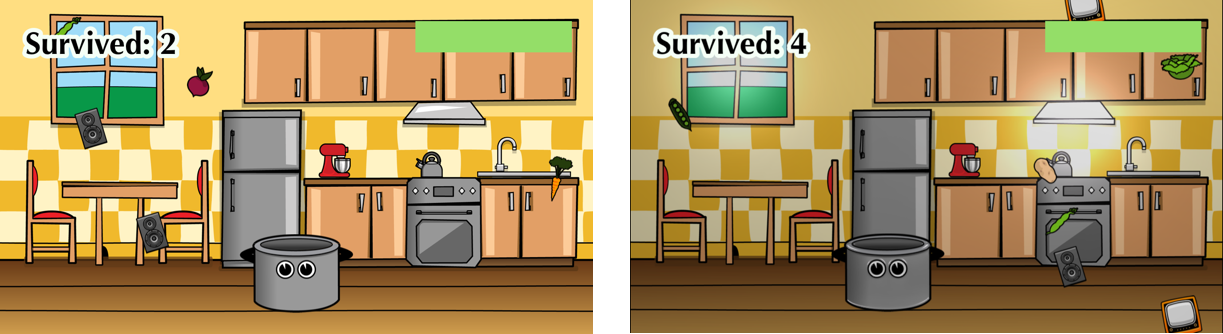
\includegraphics[width=0.9\linewidth]{images/Chapter9/lighting_comparison.png}
    \caption{Unlighted scene on the left, lighted scene on the right}
    \label{lighting_example}
\end{figure}

Most game engines require developers to write \textit{shader programs} to
use visual effects such as lighting. \cocos{} provides an API called
\inlinecode{CCEffects} that implements many common visual effects, such as
lighting, refraction, blur, etc. Using CCEffects we can enhance our games
without needing to learn how to write shader programs. 

The CCEffects can even be configured with \SB{}! We can set up all of the
lighting for this game with only a handful lines of code. 

The first step of adding lighting to our game is understanding some of the
theory that goes into lighting in 2D games.

\subsection{Lighting in 2D games}
The simplest way to light a 2D scene is to use brighter and darker colors,
depending on the distance to a given light source, I'll refer to this technique
as \textit{flat lighting}. Figure \ref{lighting_example} shows flat lighting on
the background image of our game. Some areas of the background are lighter than
others. The background is the lightest around the window and the kitchen light,
the two light sources for our game.

Flat lighting comes entirely out of the box using \cocos{}. However, using flat
lighting alone doesn't create great visual effects. In 2D games lighting can be
used to give objects a 3D feel. We are going to use that technique for the pot
and the falling objects.

We will create \textit{normal maps} for each of our game objects. A normal map
is a special kind of texture that describes the 3D surface of an object. That
way the game engine can calculate how strong certain areas of a texture should
be light up by a light source. Here's what a normal map looks like:

\begin{figure}[H]
    \centering
    
\includegraphics[width=180pt]{images/Chapter9/pot-bottom_NRM.png}
    \caption{The normal map for the bottom part of the pot. Each color encodes
    information about the object's surface}
\end{figure}

And here's a comparison that shows how lighting and normal maps together give
the pot a 3D feel:

\begin{figure}[H]
    \centering
    
\includegraphics[width=300pt]{images/Chapter9/pot_lighting_comparison.png}
    \caption{No lighting on the left, lighting with normal map on the right}
\end{figure}

The comparison above shows that certain parts of the pot appear brighter and
shinier. \cocos{} calculates the brightness for each part of the texture based
on the normal map that we provide and the position of the light. 

Lighting and normal maps for 2D games are topics that are worth dedicating
entire books to (and there are a ton out there!) so for now we will stick with
this overview of how lighting works. Even this basic knowledge will allows us to
make the game look quite a bit better. You might wonder where the normal maps
for our textures come from. The answer is: we need to create them ourselves. 

\subsection{Creating normal maps}
There are a bunch of tools available that turn creating simple normal maps into
an easy task. For this book I've provided all of the normal maps for you, as
part of the asset pack that you downloaded at the beginning of this book.

%TODO: check crazy bump license
What if you want to create normal maps for your own game? The normal maps for
this book have been created with the tool \textit{CrazyBump}
(\url{http://www.crazybump.com/}). CrazyBump uses shape detection to guess
normal maps and the results have been great for me!

If you have complicated textures, or you need to polish the lighting effects in
your game in great detail, you might want to resort to a tool that allows you to
create a normal map manually. \textit{SpriteIlluminator}
(\url{https://www.codeandweb.com/spriteilluminator}) is a great tool for
manually creating normal maps.

Since we already have all the normal maps we need, let's dive right into \SB{}
and set up some light sources!

\subsection{Setting up lighting effects in \SB{}}
Now that we have a basic understanding of 2D lighting it's time to dive into the
CCEffects API. There are three important components that we will be using:
\begin{description}
\item[CCEffectNode] is a container for all visual effects. If
you want to apply effects to \ccsprite{}s, all of them need to be the child of a
\inlinecode{CCEffectNode}. In practice this means that you'll mostly have a
\inlinecode{CCEffectNode} as a container for your entire gameplay scene.
\item[CCEffect] represents one of the different available visual effects, e.g.
lighting, refraction, blur, etc. Currently effects can only be applied to
\ccsprite{}s. You add an effect to a sprite by instantiating a
\inlinecode{CCEffect} and assigning it to a \ccsprite{}.
\item[CCLightNode] is used in combination with the effect
\inlinecode{CCEffectLighting} to define light sources.
\end{description}

To summarize what we've discussed so far: Effects can only be applied to
\ccsprite{}s. All affected sprites need to be a child of a
\inlinecode{CCEffectNode}. Light nodes are used together with the lighting
effect and define light sources. Direction and brightness of these light nodes
is used by \cocos{} to render lighting effects.

Here's a diagram of how the components play together:

\begin{figure}[H]
    \centering
    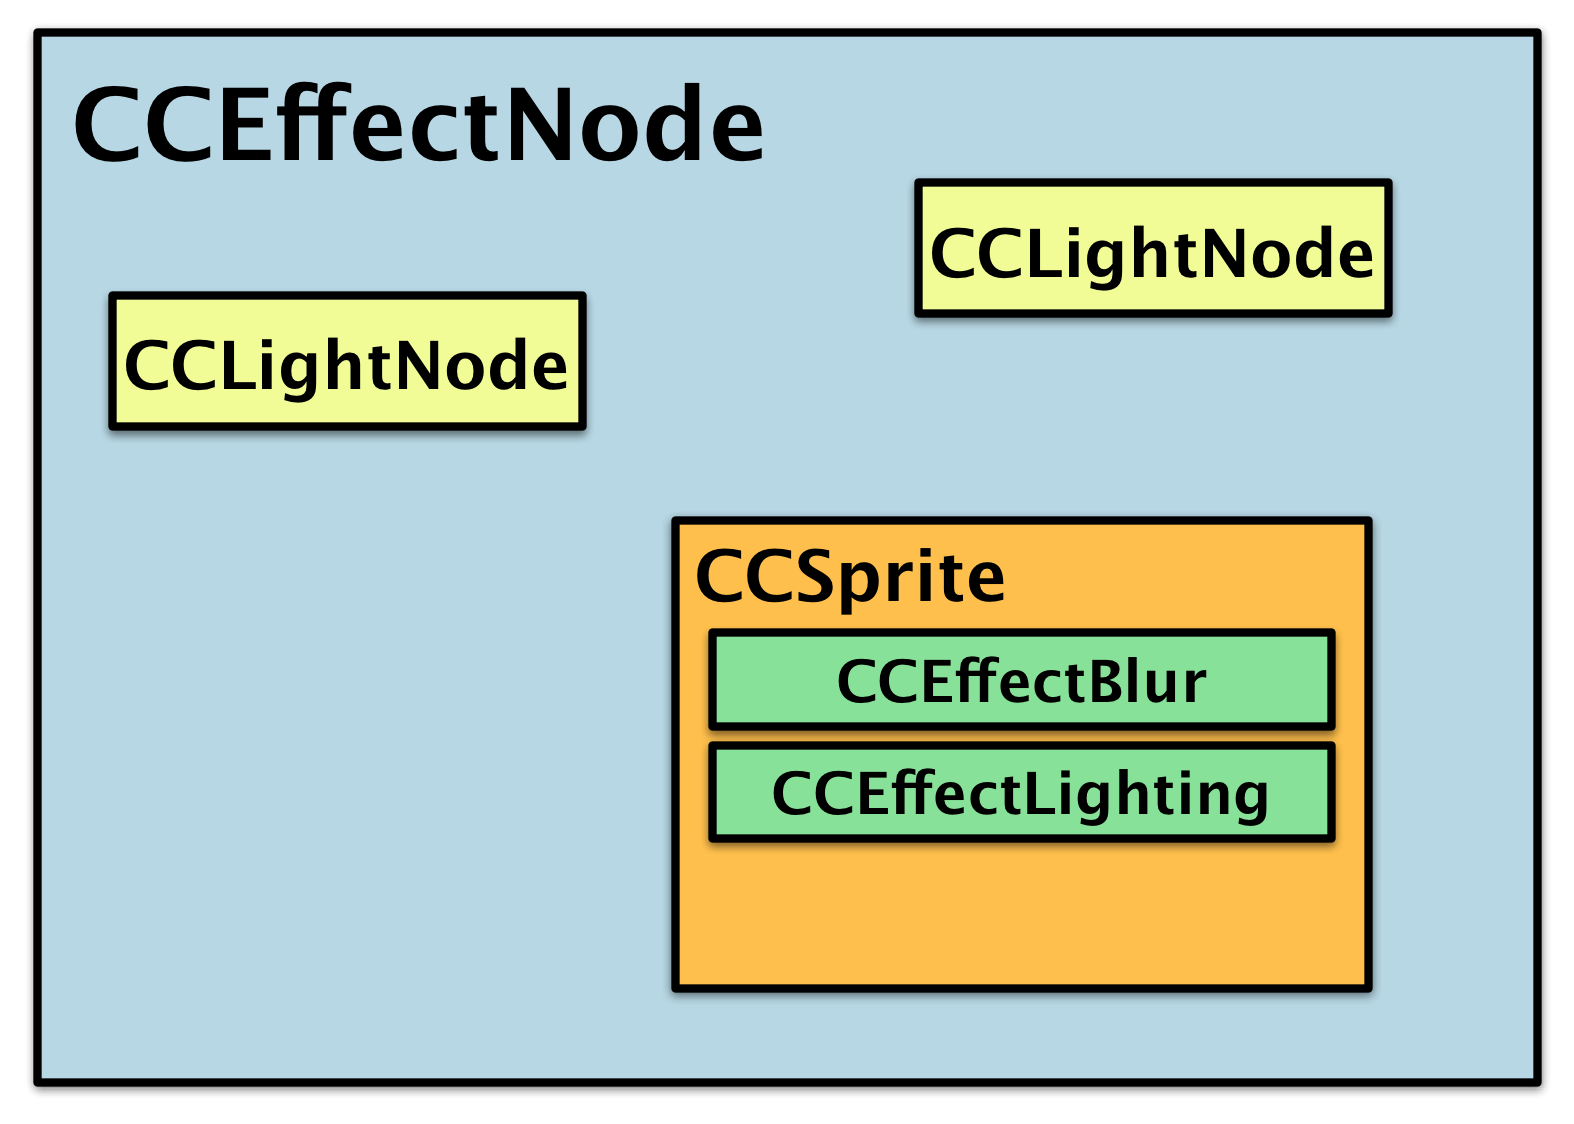
\includegraphics[width=260pt]{images/Chapter9/effect_setup.png}
\end{figure}

We will only discuss a subset of the \inlinecode{CCEffects} API, but the good
news is that it is very easy to use and therefore can be explored without much
instruction! 

There a many simple effects that can be added with a single line of
code, such as \textit{blur} or \textit{saturation}. You can add all effects in
code or in \SB{}. You can change the relevant
properties of a \inlinecode{CCEffect} in code, that
alows you to animate effects. You can for example create
a \textit{saturation} effect that starts with full
saturation and over time reduces the saturation until
the sprite turns into a grayscale image.

Finally, \inlinecode{CCEffectStack} allows you to
combine multiple effects.

\begin{details}[frametitle={More on effects}]
If you want to learn a little bit more about effects in \cocos{} you should read
our tutorial that introduces the \inlinecode{CCEffects} 
API (\url{https://www.makeschool.com/tutorials/cocos2d-3-2-with-cceffects-is-coming}).
\end{details}

This introduction gives us enough understanding to move to \SB{} and set up our
lighting. Open the \SB{} project and select the \filemention{MainScene.ccb}
file.

\begin{leftbar}
\begin{enumerate}
  \item Drag an \textit{Effect Node} from the node library to the timeline of
  \filemention{MainScene.ccb}
  \item Use the {Shift} key to select all of the nodes that are currently added
  to Main Scene: \begin{figure}[H]
    \centering
    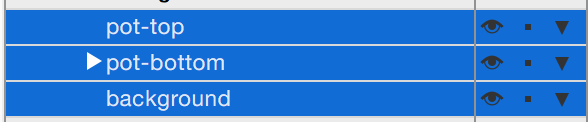
\includegraphics[width=200pt]{images/Chapter9/shift_select.png}
    \end{figure}
  \item Drag the selected nodes onto the \textit{Effect Node} to turn all of the nodes into children of the effect node. Your node
  hierarchy should look like this:
  \begin{figure}[H]
    \centering
    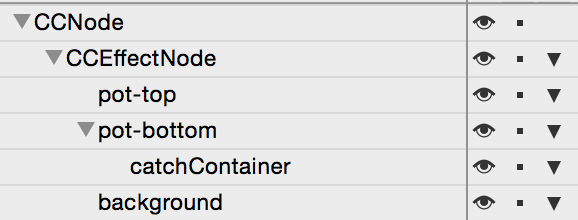
\includegraphics[width=200pt]{images/Chapter9/node_hierarchy_effect.png}
  \end{figure}
  \item Set the content size of the effect node to \textit{percentage of parent
  container} and set the size to (100\%, 100\%)
\end{enumerate}
\end{leftbar}

Now we have the \inlinecode{CCEffectNode} set up, which allows us to add visual
effects!

Next, let's look into adding the two light sources. We want the light sources to
be place on the window and above the stove. As you might remember, we are designing this game to
work on 3.5 inch iPhones, 4 inch iPhones and on iPads. 

In order to position the lights correctly for all of these device types we need
to use a little trick, simply using relative positioning with percentage values
does not work. Here's what the scene looks like on different device types using
relative positioning: 
\begin{figure}[H]
    \centering
    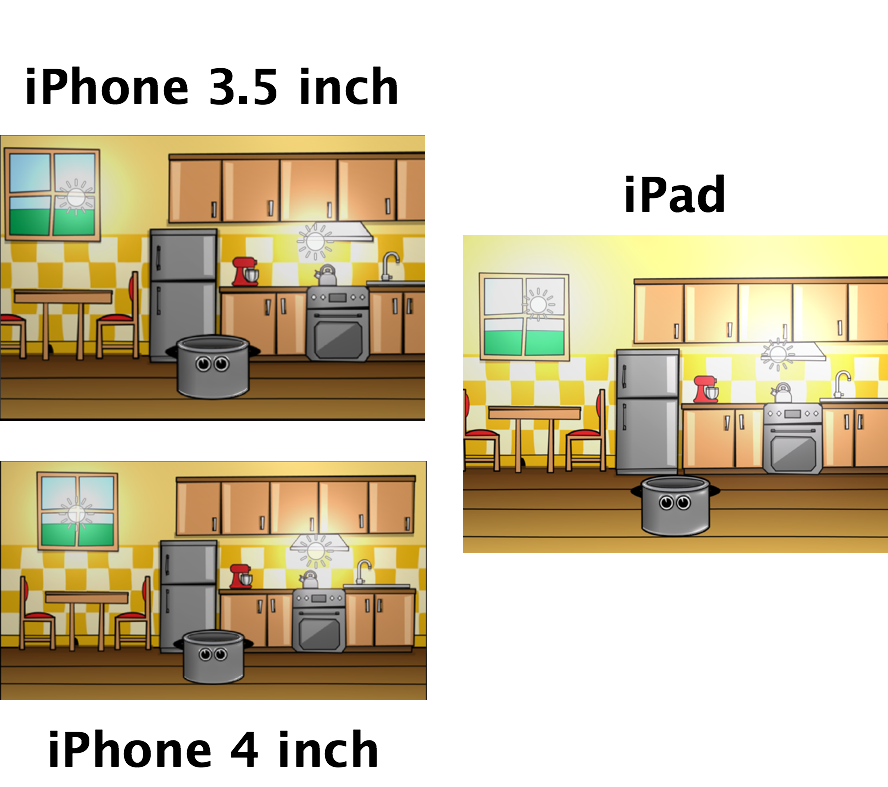
\includegraphics[width=0.8\linewidth]{images/Chapter9/light_source_relative_position.png}
    \caption{Relative positioning results in slightly different light positions
    for each device type}
\end{figure}

We have set up the background image to be centered on all device types.
Therefore the distance of the window and the stove from the screen edges varies.
This means we cannot use the screen edges as reference points for positioning
the lights.

The center of the background image is always at exactly the same position. The
trick in this situation is to position the light sources relative to that center
position. We can do so by adding an empty \ccnode{} to the center of the scene
and adding our two light sources as children.

\begin{details}[frametitle={Previewing a scene on different device types}]
We have discussed this briefly in \ref{preview_screen_sizes}, but just as a
short reminder: \SB{} allows you to preview your scenes on different device
types. To switch between different device types, go to the \textit{Document} ->
\textit{Resolution} menu:
\begin{figure}[H]
  \centering
  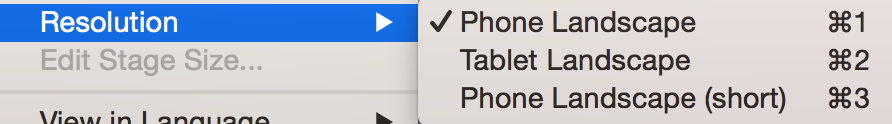
\includegraphics[width=200pt]{images/Chapter9/select_resolution.png}
\end{figure}
You can also use the shortcuts displayed next to the device types!
\end{details}
Now we can start adding the center node and the two light sources.
\begin{leftbar}
First, let's add the center node.
\begin{enumerate}
  \item Drag a plain \textit{Node} from the node library and add it as a child
  of the \textit{CCEffectNode}
  \item Set its position type to be \textit{percentage of parent container}
  \item Set the position to \textit{(50\%, 50\%)}
  \item Rename the node to \textit{light-container} by selecting the node in the
  timeline and hitting the return key
\end{enumerate}
Now we can add the light source for the window. We will discuss the interesting
properties of our light sources in detail as soon as they are set up:
\begin{enumerate}
  \item Drag a \textit{Light Node} from the node library and add it as a child
  of the \textit{CCNode} that we created just now
  \item Set the position of the light to \textit{(-180, 90)}
  \item Set the \textit{Diffuse Intensity} to \textit{0.25}
  \item Set the \textit{Specular Intensity} to \textit{0.60}
  \item Set the \textit{Ambient Intensity} to \textit{0.73}
  \item Set the \textit{Cutoff Radius} to \textit{500.00}
  \item Set the \textit{Half Radius} to \textit{0.70}
  \item Set the \textit{Depth} to \textit{180}
\end{enumerate}
And finally, add the second light source:
\begin{enumerate}
  \item Drag a \textit{Light Node} from the node library and add it as a child
  of the \textit{CCNode} that we created just now
  \item Set the position of the light to \textit{(140, 40)}
  \item Set the \textit{Diffuse Intensity} to \textit{0.20}
  \item Set the \textit{Specular Intensity} to \textit{0.60}
  \item Set the \textit{Ambient Intensity} to \textit{0.00}
\end{enumerate}
\end{leftbar}

Now you should be able to switch between the different screen sizes and see that
the lights are positioned correctly all the time! Let's discuss some of the
light properties that we just set up.

\begin{description}
\item[Diffuse Intensity] the intensity of the diffused portion of the light.
Diffused light brightens nearby objects, without resulting in a
\textit{shininess} effect. Diffused light is soft, directional light.
\item[Specular Intensity] the intensity of the specular portion of the light.
Specular light is a sharp, directional light. It causes reflections on surfaces
of objects that are lit up.
\item[Ambient Intensity] the intensity of the ambient portion of the light.
Ambient light has no direction and the distance to objects in the scene is not
relevant for this kind of light. All objects in the scene are lit up by
ambient light in exactly the same way. This factor is used to set a base
brightness.
\item[Cutoff Radius] the reach of the light in points. Only nodes within the
radius of the light will be lit.
\item[Half Radius] the portion of the radius at which the intensity of the light
has fallen to half of its maximum value. You can choose a value between 0 and 1.
A smaller value will create a sharper light, a higher value will create a
smoother light.
\item[Depth] defines the distance of the light from the pane it is lighting. A
small value means that objects are lit from the side. A large value means that
the object is far away from the pane, therefore the objects are lit from the
front.
\end{description}

The last thing to note is that \cocos{} provides two different light types:
\textit{Point lights} and \textit{Directional lights}. For this game we are only
using point lights. You can change the type in the \textit{Light type} dropdown
in the property inspector. A point light only lights up objects that are within
the cutoff radius, and objects that are further away from the light source are
lit up less than closer objects. Directional lights light up all objects in the
same way. They are similar to ambient lighting, except that the light comes from
a certain direction.

\begin{details}[frametitle={More details on lighting}]
The creator of \textit{Sprite Illuminator}, one of the normal map tools
mentioned earlier, has written a nice article on lighting in \SB{} and \cocos{}
that covers many light properties in detail: \url{https://www.codeandweb.com/blog/2015/03/17/cocos2d-dynamic-lighting-tutorial
}. The source code annotations in \filemention{CCLightNode.h} of the \cocos{}
also reveal many details about the different adjustable properties.
\end{details}

At this point we have the lighting set up, but we don't see any change in our
scene. Setting up lighting is a two step process in \cocos{}. We need to define
the light sources, which we just did. Then we need to add the \textit{Lighting
effect} to sprites that shall be effected by these light sources. In this scene
we want the background image and the bottom and top part of the pot to be
affected by our light sources.

\begin{leftbar}
\begin{enumerate}
  \item Select the \textit{background} sprite from the timeline
  \item Add a lighting effect in the property inspector as following: 
  \begin{figure}[H]
    \centering
    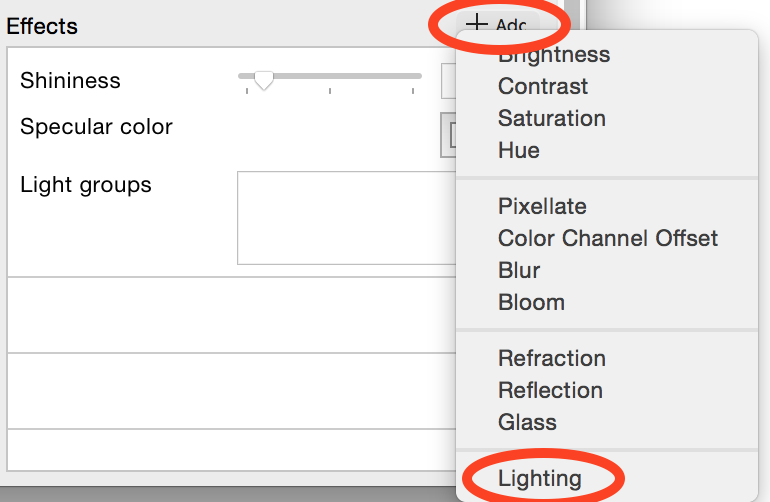
\includegraphics[width=200pt]{images/Chapter9/add_lighting_effect.png}
  \end{figure}
  \item Select \textit{pot-top} and add a lighting effect in the same way you
  added it to the background
  \item Adjust the \textit{shininess} of this lighting effect to \textit{0.3}
  \item Select \textit{pot-bottom} and add a lighting effect
  \item Adjust the \textit{shininess} to \textit{0.3} 
\end{enumerate}
\end{leftbar}

Now you should see the lighting taking effect! The last thing we need to do is
add our normal maps.

\subsection{Assigning normal maps in \SB{}}
Now that our light sources and lighting effects are set up, let's assign the
normal maps to our sprites so that we get more detailed lighting. For the \textit{pot-top}
and \textit{pot-bottom} sprite, we can set up the normal map in \SB{}. The
falling objects are spawned dynamically in code, we will look at how to set up
their normal maps in the next section.

Adding normal maps to sprites is very simple in \SB{}. In the property
insepctor of a \ccsprite{} there's a separate dropdown below the \textit{Sprite
frame} dropdown that allows us to assign a normal map:

\begin{figure}[H]
  \centering
  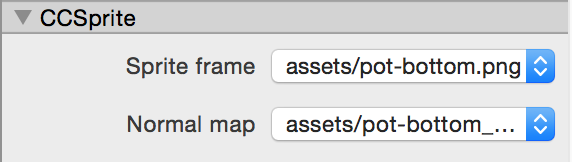
\includegraphics[width=200pt]{images/Chapter9/select_normal_map.png}
\end{figure}

\begin{leftbar}
\begin{enumerate}
  \item Select \textit{pot-top} in the timeline 
  \item Set the normal map to \filemention{assets\/pot-top\_NRM.png}
  \item Select \textit{pot-bottom} in the timeline
  \item Set the normal map to \filemention{assets\/pot-bottom\_NRM.png}
\end{enumerate}
\end{leftbar}

Great! Now you should see a nicely lit scene, with subtle reflections on the
pot:

\begin{figure}[H]
  \centering
  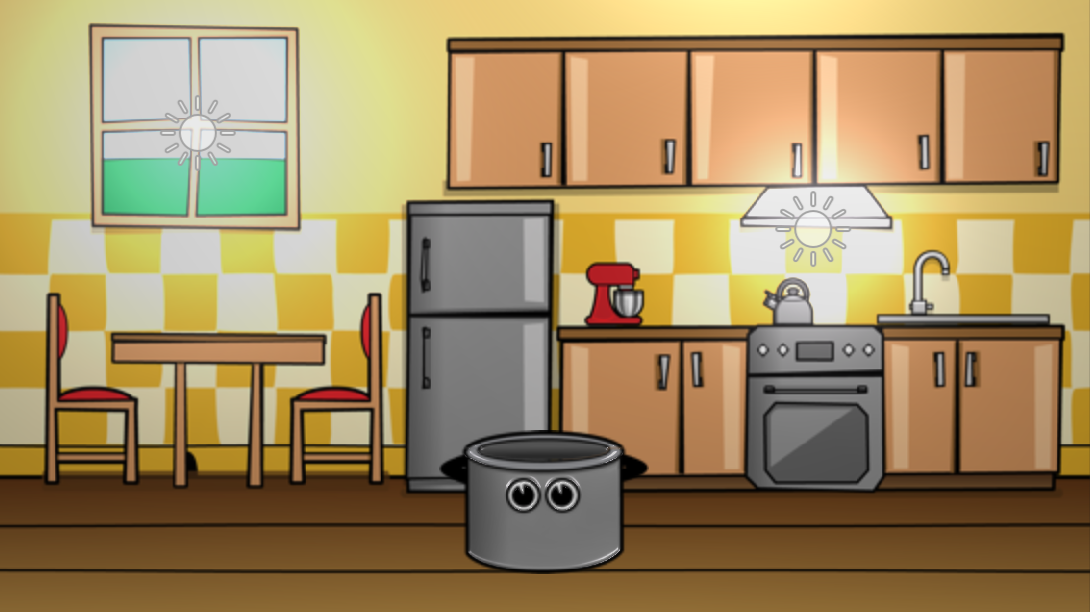
\includegraphics[width=350pt]{images/Chapter9/lighting_finished.png}
\end{figure}

Note that the preview of the lighting effects in \SB{} currently don't match the
lighting effects on the simulator or device exactly. To get a good understanding
of how your lighting effects are working you'll need to run your game from
\xcode{}.

Now all that's left in terms of lighting is assigning normal maps to
our falling objects as well!

\begin{details}[frametitle={Testing lighting effects on the simulator}]
In case you've been curious and have tried running the current version of the
project, you might have realized that the performance in the simulator is
extremely poor. The reason is that the iOS simulator doesn't use your computers
GPU for all OpenGL features, but instead simulates many of them in software,
which in many cases can be extremely slow. When working with CCEffects, I highly
recommend testing your game on an actual device, even though that means that
you're required to purchase an Apple Developer license.
\end{details}

\subsection{Assigning normal maps in code}
As mentioned earlier, the falling objects are spawned dynamically in code,
therefore we cannot assign the normal maps in \SB{}. However, adding normal
maps in code is pretty simple. Additionally we will also need to look into
adding the lighting effect to all falling objects in code, so that they are
affected by our two light sources.

As you might remember, we had a clever way of managing the different assets for
our falling objects. We are using a \textit{plist} file that stores the image
names for all \textit{positive} and \textit{negative} objects. The goal of this
attempt is to keep information about game content outside of our codebase. In
software design this principle is called \textit{configuration over code}.

Ideally we want to use the same approach for the normal maps we are about to
assign. We could simply add the image names of all the normal maps to the plist
to accomplish that. However, there's another interesting principle in software
design: \textit{convention over configuration}. When creating the normal maps
for the sprites in our game, I have followed a \textit{convention}. Each normal
map file name is built as following: \textit{\{ImageName\}\_NRM.png}

This means that we know the file name of the normal map as soon as we now the
file name of the sprite's texture. Using this knowledge, the implementation of
setting up normal maps in code becomes pretty straightforward.

\begin{leftbar}
Open \filemention{FallingObject.swift} and extend the \inlinecode{init(type:)}
initializer by adding the following lines \textbf{to the end of the
initializer}:
\begin{lstlisting}
effect = CCEffectLighting()
    
let imageNameSplit = split(imageName!) { $0 == "." }
let imageNameFirstPart = imageNameSplit[0]
let normalMapName = "\(imageNameFirstPart)_NRM.png"

normalMapSpriteFrame = CCSpriteFrame.frameWithImageNamed(normalMapName) as! CCSpriteFrame
\end{lstlisting}
\end{leftbar}

By adding the code above to the initializer of \inlinecode{FallingObject}, we
make sure that the lighting effect and the normal map are set up as soon as the
object is created.

In the first line we set up the \inlinecode{CCEffectLighting} and assign it to
the \inlinecode{effect} property of our \inlinecode{FallingObject}. The
\inlinecode{effect} property is inherited from \inlinecode{CCSprite}. Now our
falling object will be affected by light sources.

The remaining lines are used to assign the correct normal map to this object. We
split the image name to get the part before the file extension. Then we append
\textit{\_NRM.png} to that first part to retrieve the filename of the normal
map. Within the closure passed to the \inlinecode{split} function we access a
variable called \inlinecode{\$0}. This is a cool feature in Swift, within
closures we can access parameters either by name or by using the \inlinecode{\$}
symbol in combination with the index of the argument. Using these shorthand
argument names is pretty common when working with standard library functions
such as \inlinecode{split}, \inlinecode{map}, etc.

Finally we use that filename to load a \inlinecode{CCSpriteFrame} that we can
assign to the \inlinecode{normalMapSpriteFrame}. That property is also inherited
from \inlinecode{CCSprite}.

Now our falling objects are good to go! If you run this version of the game you
should see detailed lighting effects and subtle reflections on all of the
spawned objects.

This concludes our coverage of the \inlinecode{CCEffects} API for this book. You
now know the basic set up that effects require. You also know how to configure
effects in \SB{} and in code. The lighting effect is one of the more complicated
ones provided by the effects API - you should be able to pick up simpler effects
such as blur and saturation pretty easily.

If you find some time, I highly recommend playing around with this API. With
little time investment you will be able to create stunning visual effects.

\section{Adding Particle Effects}
Another great way to improve the look and feel of your app is to add particle
effects. Particle effects are used to animate huge amounts of very small
sprites, which can be very useful when animating fire, smoke or explosions.
Here's an example of what a particle effect in \cocos{} can look like:

\begin{figure}[H]
  \centering
  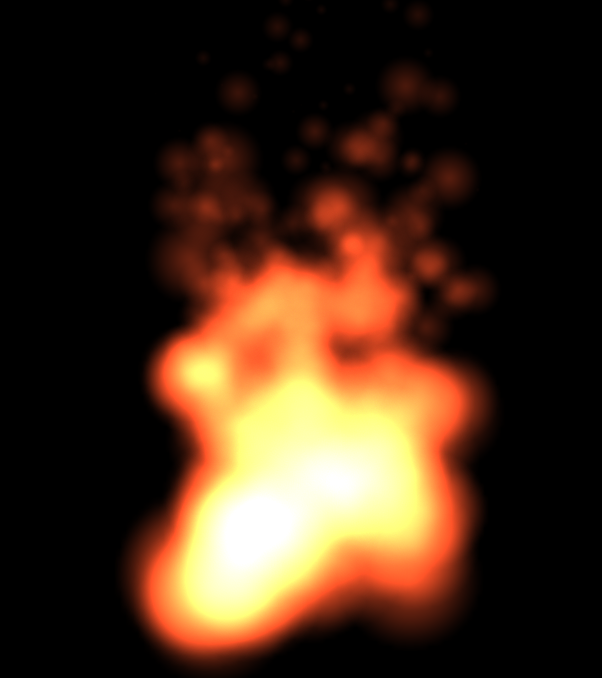
\includegraphics[width=130pt]{images/Chapter9/particle_fire.png}
\end{figure}

\SB{} comes with built in support for particle effects which makes it easy to
create them and iterate on them while watching a live visual preview. 
For our game we will add a particle effect that takes place as soon as the
player catches one of the good objects.

We are going to create the particle effect in \SB{}, then load it and add it to
the scene dynamically in code.

\subsection{Creating a Particle Effect in \SB{}}
Let's open our \SB{} project to get started!

\begin{leftbar}
Create a new \ccbfile{} of type \textit{Particle} and call it
\textit{CaughtParticleEffect.ccb}:
\begin{figure}[H]
  \centering
  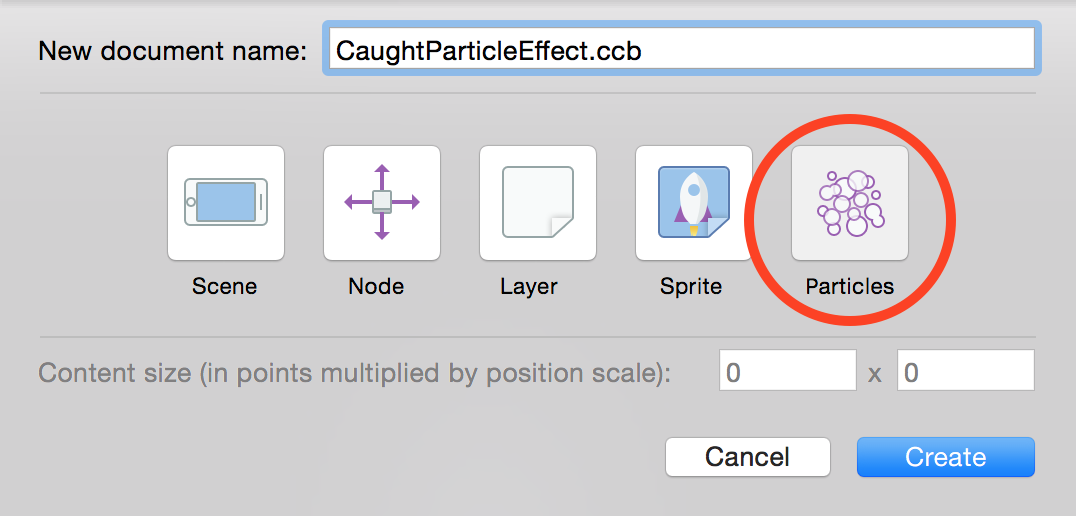
\includegraphics[width=250pt]{images/Chapter9/create_particle_effect.png}
\end{figure}
\end{leftbar}

Now you should see a new file with the default fire particle effect. We want to
use a different effect for our game.

Now how do we go about building our explosion effect? There are two different
aspects that make up a particle effect. The first is the texture for the
individual particles, the second are all the settings that define how the
particles of the system move, change over time, how long the entire particle
systems lasts, etc. There are well over 20 settings that you can use to build
your particle effects - discussing all of them goes well beyond the scope of
this book.

There are two essentially different ways to start out building your own effect.
You can start entirely from scratch, choosing your own particle texture and
experimenting with the vast amount of available configuration options.
Alternatively you can select a particle effect from \SB{} templates and modify
it to build your custom effect.

In most cases this second approach makes more sense. You will likely be able to
find an existing particle effect that is a good starting point for your
custom one. For this game we will use that second approach and will use a very
slightly modified library effect.

The best way to dive deeper into particle effects is spending some time playing
around with the different options the editor in \SB{} provides.

Let's turn our fire effect into an explosion effect.

\begin{leftbar}
Select the \textit{CCParticleSystem} in the timeline. Then open the last tab in
the inspector panel on the right. Scroll down to the \textit{Exploded Ring}
effect and \textbf{double-click} onto it to select it:

\begin{figure}[H]
  \centering
  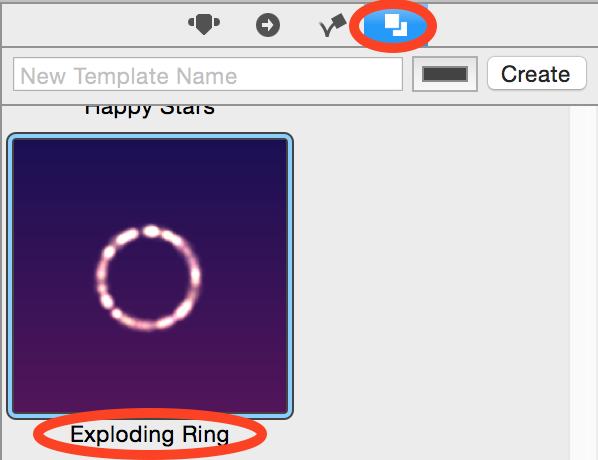
\includegraphics[width=250pt]{images/Chapter9/select_exploded_ring.png}
\end{figure}
\end{leftbar}

Now you should see the fire being replace by an exploding ring. You will notice
that this particle effect will only run once, then you will see a blank stage.
That's because this template creates an effect in which has a limited lifetime.
The fire effect had a \textit{duration} of \textit{-1.0} seconds which indicates
an endlessly looping effect. This effect has a \textit{duration} of \textit{0.01}
which means that particles are only emitted for a very short time. If you
want to see what the particle effect looks like again, you can click the
\textit{Start Particles} in the inspector panel. 

The \textit{duration} property defines the lifetime of the particle system,
which defines how long particles will be created.

Each individual particle has a lifetime as well. In the exploded ring template
the lifetime is set to \textit{1.0} seconds. The larger this value, the longer
the particles stay visible as the move from the center to the edge of the stage.
This makes the ring appear larger. 

We actually want the ring to be a little bit smaller. Later we will add it to
the inside of the pot as soon as an object is caught. We want it to look like
all the particles are contained inside of the pot. After playing around with a
few values I settled with \textit{0.6} for the lifetime of each particle.

\begin{leftbar}
Change the \textit{Life} property of this effect in the inspector
panel to \textit{0.6}:
\begin{figure}[H]
  \centering
  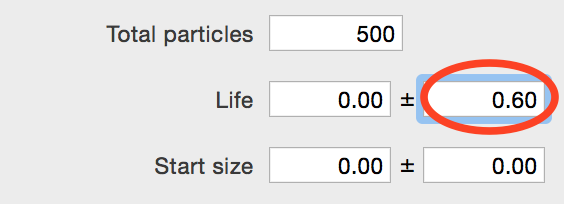
\includegraphics[width=250pt]{images/Chapter9/change_lifetime.png}
\end{figure}
\end{leftbar}

When you start this particle effect again you will see that the explosion circle
now appears smaller. This completes our particle effect setup in \SB{}. Feel
free to spend some time exploring the other properties of particle effects
before moving on.

Next, we'll load this particle effect in code and add it to our game scene
dynamically whenever the user catches a good object!

\subsection{Loading particle effects in code}
Now it's time to pull up the \xcode{} project again. We want to run the particle
effect when the player catches a good object. This means we need to extend the
\inlinecode{performCaughtStep} method that we implemented earlier.

We'll first load the \ccbfile{} that stores the particle effect, then we
position it and add it to the top part of the pot, this will make the effect
appear to take place inside of the body of the pot. The particle effect starts
automatically, as soon as it is added to a visible scene.

Let's implement this feature and then discuss some more details!

\begin{leftbar}
Extend the implementation of \inlinecode{performCaughtStep(fallingObject:)} to
load and add the particle effect:
\begin{lstlisting}
func performCaughtStep(fallingObject:FallingObject) {
  // if the object was caught, remove it as soon as soon as it is entirely contained in the pot
  if (CGRectContainsRect(catchContainer.boundingBox(), fallingObject.boundingBox())) {
    gameModeDelegate?.gameplay(self, caughtFallingObject: fallingObject)
    fallingObject.removeFromParent()
    let fallingObjectIndex = find(fallingObjects, fallingObject)!
    fallingObjects.removeAtIndex(fallingObjectIndex)
    
    if (fallingObject.type == .Good) {      
      let particleEffect = CCBReader.load("CaughtParticleEffect") as! CCParticleSystem
      particleEffect.autoRemoveOnFinish = true
      particleEffect.positionType = CCPositionType(
        xUnit: .Normalized,
        yUnit: .Points,
        corner: .TopLeft
      )
      particleEffect.position = ccp(0.5, 20)
      potTop.addChild(particleEffect) 
    }
    
  }
}
\end{lstlisting}
\end{leftbar}
Let's look at the code we added, step by step. First, we check the object type.
We want to display the particle effect only if the user caught a
\inlinecode{.Good} object. If that's the case, we use the \inlinecode{CCBReader}
to load the \ccbfile{} that contains the particle effect. We parse the value
returned by the \inlinecode{CCBReader}.

Next, we configure an important setting on the particle effect. We set
\inlinecode{autoRemoveOnFinish} to \inlinecode{true}. This means that \cocos{}
will take care of removing this particle effect from its parent object as soon
as the particle effect completed. A particle effect completes once all emitted
particles have reached the end of their lifetime. Without this line of code you
would need keep track of all added particle effects manually and make sure to
remove them - an easy way to introduce memory issues.

With the particle loaded and set up, we take care of positioning it. This
particle effect should be rendered inside of the pot's body. I've decided to
center the effect horizontally. We set up a position type that makes the
centering easy and that allows us to position the particle effect from the top
edge of the top instead of from the bottom.

Then we set the position: horizontally centered, vertically slightly below the
top edge of the pot.

In the last step we add the \inlinecode{particleEffect} to \inlinecode{potTop}.

\begin{details}[frametitle={An alternative positioning approach}]
Instead of setting the position type and the position of the particle system in
code, you could also add an empty node in \SB{} at the position where you want
to render the particle effect. Then you could add the particle effect to that
node instead of to \inlinecode{potTop}. I tend to use this approach for
positions that are harder to express in code.
\end{details}

Now you can run the game. You'll see the particle effect run as soon as you
catch a good object. This game is already looking a lot more polished than at
the beginning of this chapter.

In the next and last section we will look into using the \SB{} timeline to add
some more animations to our core gameplay.

\section{Delightful animations with \SB{}'s timeline}
We will now add some animations to the game to wrap this chapter up. So far
we've used the \SB{} timeline to animate user interfaces, now we want to
animate parts of our gameplay as well.

Whenever the player catches a good object we'll let the pot play a little wobble
animation:

\begin{figure}[H]
  \centering
  
\includegraphics[width=0.8\linewidth]{images/Chapter9/wobble_animation.png}
\end{figure}

Later on we will create a second animation based on this one where we add a
coloring effect that turns the pot red. We will use that second animation
whenever the user catches a bad object.

%TODO: check why it is fine to add spawning objects to Main while pot is added
% to effect node
Let's get started on creating these animations! You might remember that the top
and the bottom part of the pot need to have the same parent node as the falling
object due to a limitation in \cocos{}. This means we cannot group them under
a container node. We discussed this in detail in chapter \ref{rendering_tweak}
(\textit{A rendering tweak}). This unfortunately means that we need to copy the
keyframes for the animation for both parts of the pot. Luckily \SB{} makes this
pretty easy!
\begin{leftbar}
Open up the \SB{} project and select the \filemention{MainScene.ccb} file. 
\begin{enumerate}
  \item Create a new timeline
  \item Name that timeline \textit{CatchAnimation}: 
  \begin{figure}[H]
  \centering
  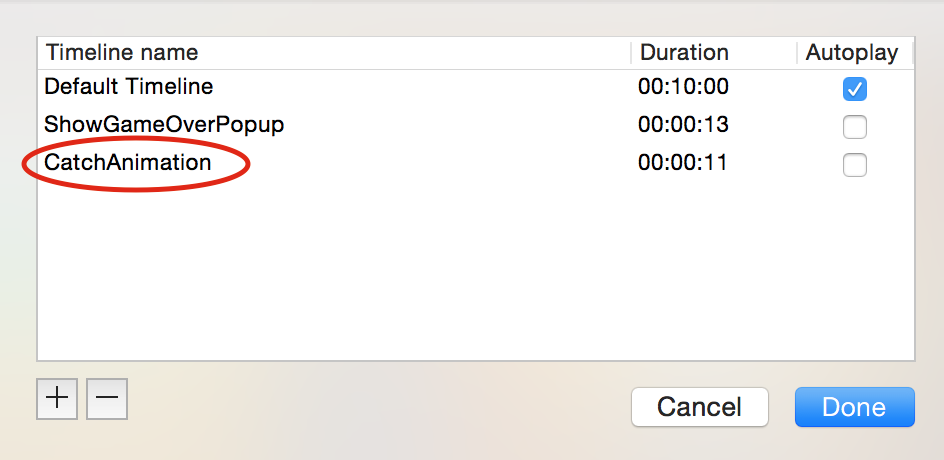
\includegraphics[width=300pt]{images/Chapter9/rename_timeline.png}
  \end{figure}
  
  \item Zoom in all the way in the timeline since the animation we're building
  will be very short:
  \begin{figure}[H]
  \centering
  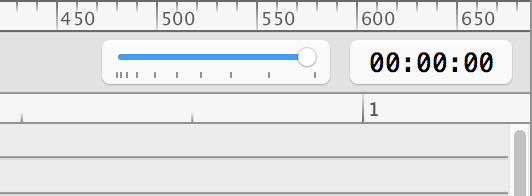
\includegraphics[width=300pt]{images/Chapter9/zoom_timeline.png}
  \end{figure}
\end{enumerate}
\end{leftbar}
 
